 \section{Case Studies}
\label{sec:case_study}
To demonstrate the effectiveness of the Safety Annex, we describe two case studies.

\begin{figure*}[!ht]
	\begin{center}
		%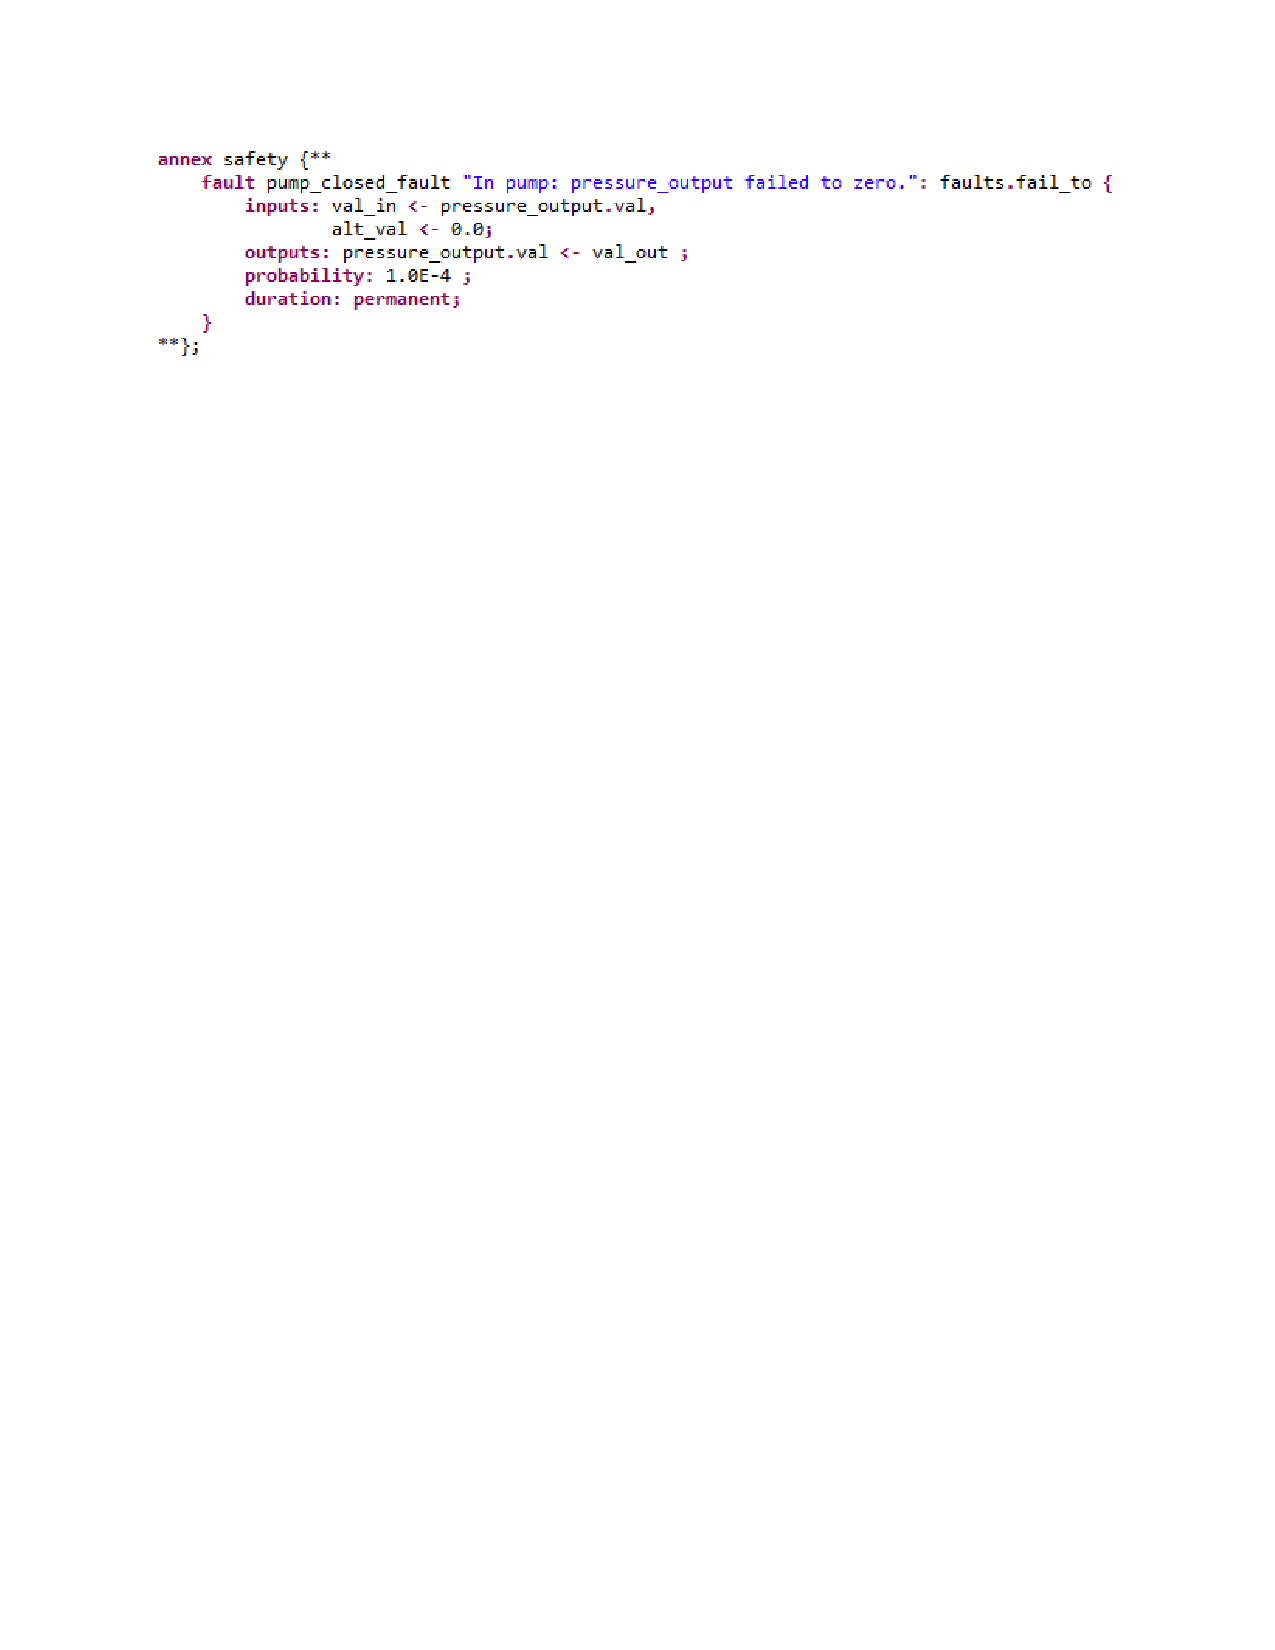
\includegraphics[trim=0 330 150 0,clip,width=1.0\textwidth]{images/pump_fault.png}
		\vspace{-50pt}
		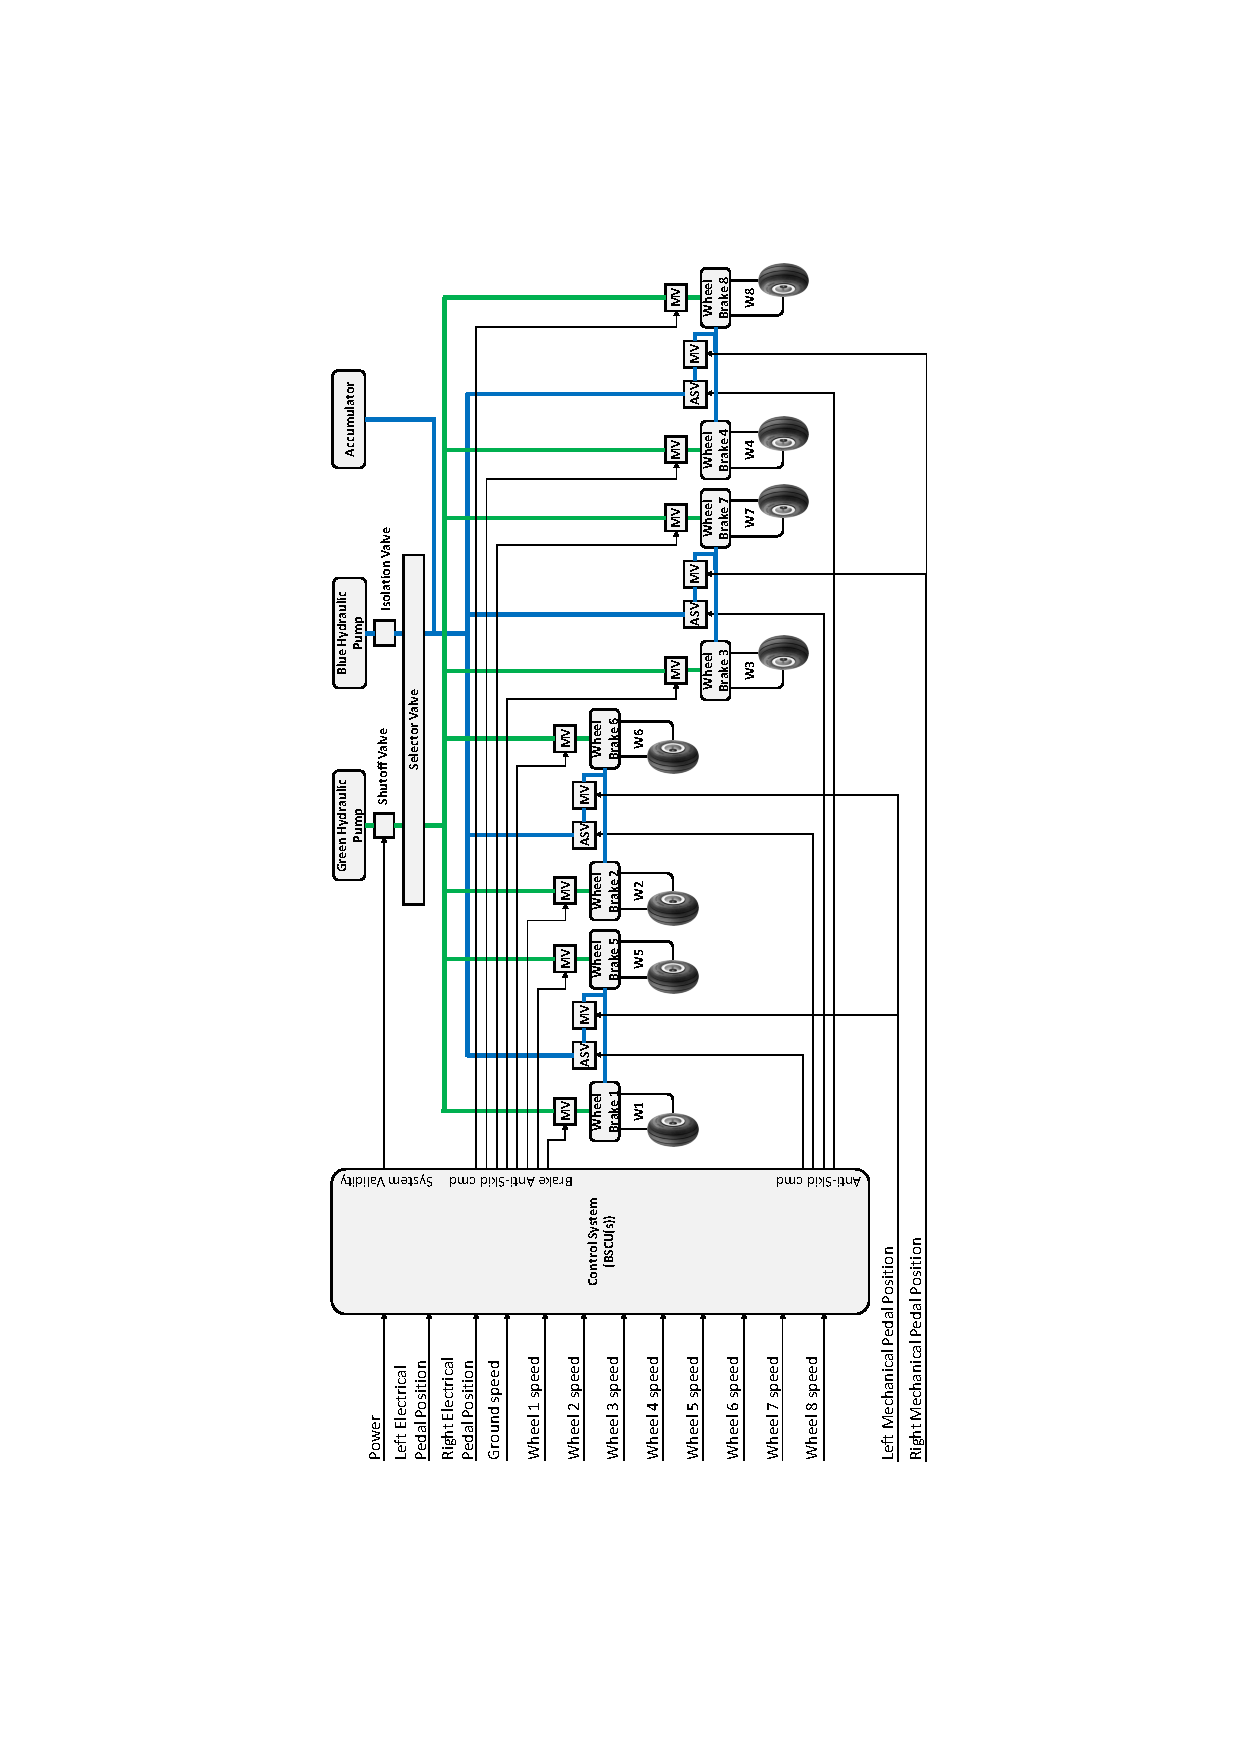
\includegraphics[trim=20 20 20 20,clip,width=1.0\textwidth]{images/wbs_large.pdf}
		\vspace{-70pt}
		\caption{High Level Wheel Brake System}
 		\label{fig:wbs1}
	\end{center}
\end{figure*}

\subsection{Wheel Brake System}
The Wheel Brake System (WBS) described in AIR6110~\cite{AIR6110} is a well-known example that has been used as a case study for safety analysis, formal verification, and contract based design~\cite{DBLP:conf/cav/BozzanoCPJKPRT15, 10.1007/978-3-319-11936-6-7, CAV2015:BoCiGrMa, Joshi05:SafeComp, mattarei}. The preliminary work for the safety annex used a simplified model of the WBS~\cite{Stewart17:IMBSA}. In order to demonstrate scalability of our tools and compare results with other studies, a functionally and structurally equivalent AADL version was constructed of one of the most complex WBS xSAP models (arch4wbs)~\cite{DBLP:conf/cav/BozzanoCPJKPRT15}. 

The Aerospace Information Report 6110 (AIR6110) document provides an example of a single aircraft system, namely the braking system, for the hypothetical passenger aircraft model S18. The two engine passenger aircraft is designated to carry up to 350 passengers for an average flight time of 5 hours. The purpose of the system is to provide a clear example of systems development and its analysis using the methods and tools described in ARP4754A/ED-79A. This brake system implements the aircraft function \textit{''Decelerate aircraft on the ground (stopping on the runway)"}. The wheel brake system architecture is shown in Figure~\ref{fig:wbs1} and is taken from the work of Mattarei~\cite{mattarei}. 

\subsubsection{WBS overview and architecture description}
The WBS is a hydraulic braking system that provides braking of left and right landing gears, each of which have four wheels. Each landing gear can be individually controlled by the pilot through left/right brake pedals. 

The WBS is composed of two main parts: the control system and the physical system. The control system electronically controls the physical system and contains a redundant Braking System Control Unit (BSCU) in case of failure. In addition to the redundant BSCU channel, the control system is composed of a number of logical components including sensors for the wheels and brake pedal position, a monitor system that checks validity of the BSCU channel, and the command system which commands braking for each of the 8 wheels. The control system is primarily used in the normal mode of operation to command brake pressure.  

The physical system consists of the hydraulic circuits running from hydraulic pumps to wheel brakes. This circuit contains the pumps for both normal and alternate modes of operation (named green and blue lines respectively), a selector valve which selects the circuit depending on input from the BSCU, meter valves at each wheel. These are the physical components that provide braking force to the 8 wheels of the aircraft.

There are three operating modes in the WBS model. In \textit{normal} mode, the system uses the \textit{green} hydraulic circuit. In the normal mode of operation, the selector valve uses the green hydraulic pump to supply fluid to the wheels. Each of the 8 wheels has one meter valve which  are controlled through electronic commands coming from the BSCU. These signals provide brake commands as well as antiskid commands for each of the wheels. The braking command is determined through a sensor on the pilot pedal position. The antiskid command is calculated based on information regarding ground speed, wheel rolling status, and braking commands.

In \textit{alternate} mode, the system uses the \textit{blue} hydraulic circuit.  The wheels are all \textit{mechanically} braked in pairs (one pair per landing gear). The alternate system is composed of the blue hydraulic pump, four meter valves, and four antiskid shutoff valves. The meter valves are mechanically commanded through the pilot pedal corresponding to each landing gear. If the system detects lack of pressure in the green circuit, the selector valve switches to the blue circuit. This can occur if there is a lack of pressure from the green hydraulic pump, if the green hydraulic pump circuit fails, or if pressure is cut off by a shutoff valve. If the BSCU channel becomes invalid, the shutoff valve is closed.

The last mode of operation of the WBS is the \textit{emergency} mode. This is supported by the blue circuit but operates if the blue hydraulic pump fails. The accumulator pump has a reserve of pressurized hydraulic fluid and will supply this to the blue circuit in emergency mode.

The model contains 30 different kinds of components, 169 component instances, a model depth of 5 hierarchical levels.  The model includes one top-level assumption and  11 top-level system properties, with 113 guarantees allocated to subsystems.  There are a total of 33 different fault types and 141 fault instances within the model.  The large number of fault instances is due to the redundancy in the system design and its replication to control 8 wheels. 

An example property is to ensure no inadvertent braking of each of the 8 wheels.  This means that if all power and hydraulic pressure is supplied (i.e., braking is commanded), then either the aircraft is stopped (ground speed is zero), or the mechanical pedal is pressed, or brake force is zero, or the wheel is not rolling.


\subsubsection{Fault Analysis of WBS using Safety Annex}

Fault analysis on the top level WBS system was performed on the 11 top-level properties using two fault hypotheses.  In the first case, we allow at most one fault, and in the second we allow combinations of faults that exceed the acceptable probability for the top-level hazard defined in AIR6110.

We use this model to illustrate the use of formal fault analysis and to show the scalability of our tools.  We applied both {\em monolithic} analysis, in which the entire model is flattened and analyzed at once, and also {\em compositional} analysis, where each architectural layer is analyzed hierarchically.
For the fault-free ``nominal'' system model, monolithic analysis requires 21 seconds, whereas compositional analysis requires 1 minute and 53 seconds.  Although the compositional time is longer, each sub-problem completes in less than 5 seconds.  The additional time for compositional analysis is  due to the start-up overhead to invoke the JKind model checker many times for individual layers.  On the other hand, when examining the model under a single-fault hypothesis (maximum one fault present in the system), compositional analysis requires 2 minutes 6 seconds, while monolithic analysis did not terminate after 60 minutes. The reason for this lies in the difference between compositional analysis and monolithic analysis as described in Section~\ref{subsec:agree}. 

Given a probabilistic fault hypothesis of $5*10^{-7}$, monolithic analysis requires 3 minutes 25 seconds.

During our analysis, we discovered that most properties were verified, but the \textit{Inadvertent braking at the wheel} properties are not resilient to a single fault nor do they meet the desired $10^{-9}$ fault threshold for probabilistic analysis.  In our model (as in the NuSMV model~\cite{DBLP:conf/cav/BozzanoCPJKPRT15}), there is a single pedal position sensor for the brake pedal.  If this sensor fails, it can command braking without a pilot request.  Given the counterexample returned by the tools, it is straightforward to diagnose the fault conditions that lead to property failure.

This counterexample can be used to further analyze the system design.  For our model, there are several possible reasons for failure: it could be that that redundant sensors are required on the pedals (here we note that the architecture of the pedal assembly is not discussed in AIR6110), or that the phase of flight is sufficiently short that we need to adjust our pedal failure rate to match this phase of flight, rather than normalizing the failure rate to per-flight-hour.  It is straightforward and computationally inexpensive to run the analysis, allowing quick iterations between systems and safety engineers. The sync and update between the preliminary system artifact analysis (FTA, etc.) and the architecture model continues until the system safety property is satisfied with the desired fault tolerance and failure probability achieved.

\subsection{Quad-Redundant Flight Control System}
\label{subsec:qrfc_case_study}
We have also used the Safety Annex to examine more complex fault types, such as {\em Byzantine} faults.  A Byzantine fault presents different symptoms to different observers, so that they may disagree regarding whether a fault is present. For example, a sensor may appear to be both failed and functional to different components to which it provides signal. 

The Quad-Redundant Flight Control System (QFCS) was first developed in Simulink and then manually translated in AADL by Backes, et. al. This system consists of four cross-checking flight control computers (FCC). The work done by Backus formalized the requirements for components of the system and for more detail on the requirements specification, see the original paper~\cite{QFCS15:backes}. 

The QFCS nominal system model was extended to model and analyze various types of faulty behaviors. Faulty behaviors were introduced to analyze the response of the system to multiple faults, and to evaluate fault mitigation logic in the model. As expected, the QFCS system-level properties failed when unhandled faulty behaviors were introduced.

We also used the Safety Annex to explore more complicated faults at the system level on a simplified QFCS model with cross-channel communication between its Flight Control Computers.

\begin{itemize}
	\item Byzantine faults were simulated by creating one-to-one connections from the source to multiple observers so that disagreements could be introduced by injecting faults on individual outputs~\cite{Driscoll-Byzantine-Fault}. The system level property ``at most one flight control computer in command'' was falsified in one second in the presence of Byzantine faults on the baseline model. The same property was verified in three seconds on an extended model with a Byzantine fault handling protocol added.  System designers can use this approach to verify if a system design is resilient to Byzantine faults, examine vulnerabilities, and determine if a mitigation mechanism works.
	
	\item Dependent faults were modeled by first injecting failures to the cross-channel data link (CCDL) bus (physical layer), and faults to the flight control computer (FCC) outputs (logical layer), then specifying fault propagations in the top level system implementation (where the data connections between FCC outputs were bound to the CCDL bus subcomponents). The fault propagation indicates that one CCDL bus failure can trigger all FCC output faults. With the fault hypothesis that allows a maximum of one fault active during execution, the system level property ``not all FCCs fail at the same time'' was falsified in one second.
	
	
\end{itemize}
\newpage
